\section{Test procedure and results}\label{sec:tests}
\subsection{Frequency measurement}\label{sec:test-freq}
\subsubsection{Lower limit}
The timer used for frequency measurement has a 32-bit counter.
Operating at \SI{48}{\mega\hertz}, the time before counter overflow is:
\begin{align*}
  {2^{32} -1 \over \SI{48}{\mega\hertz}} \approx \SI{89.48}{\second}.
\end{align*}
This corresponds to a minimum frequency of \SI{0.0112}{\hertz}.
This value was confirmed by using a function generator to create a square pulse with a \SI{90}{\second} period and observing the ``Timer period overflow'' message on the console.

\subsubsection{Upper limit}
We were able to determine the ISR overhead by sending high frequency signals to the microcontroller and checking the elapsed clock cycles between interrupts.
It was not possible to exit and re-enter the ISR in fewer than 61 clock cycles.
At \SI{48}{\mega\hertz} this corresponds to \SI{1.27}{\micro\second} of overhead or \SI{787}{\kilo\hertz}.
Indeed, input frequencies lower than \SI{787}{\kilo\hertz} had more than 61 clock cycles of overhead, confirming that 61 is the minimum overhead.

The error in the measured frequency can be expressed as:
\begin{align}\label{eqn:freq-error}
  {f \cdot 61 \over \SI{48}{\mega\hertz}} \times 100 \%
\end{align}
Using the minimum and maximum 555 timer frequency values from Section~\ref{sec:test-timer} in \eqref{eqn:freq-error} gives the range of error on the measured signal as \SIrange{0.0972}{0.142}{\percent}.

The Nyquist sampling limit, $f_s = {1 \over 2} f_{max} = \SI{24}{\mega\hertz}$, is not relevant because the upper limit from the overhead applies well before the sampling limit.

\subsection{Timer output}\label{sec:test-timer}

\begin{figure}[htpb]
  \centering
  \subfigure[Potentiometer at \SI{0}{\ohm}]
  {
    \label{subfig:pot-low}
    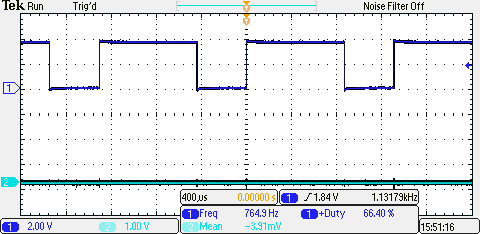
\includegraphics[width=0.475\linewidth]{../graphics/pot-low}
  }
  \subfigure[Potentiometer at \SI{5}{\kilo\ohm}]
  {
    \label{subfig:pot-high}
    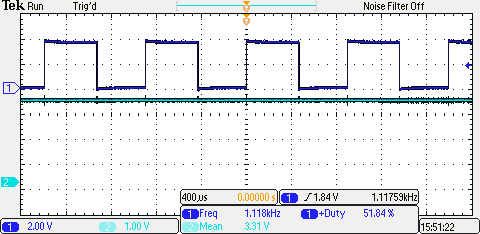
\includegraphics[width=0.475\linewidth]{../graphics/pot-high}
  }
  \caption{Timer output (top, PA1) and potentiometer voltage (bottom, PA0)}
  \label{fig:pot-traces}
\end{figure}

\begin{figure}[htpb]
  \centering
  \subfigure[Potentiometer at \SI{0}{\ohm}]
  {
    \label{subfig:opto-low}
    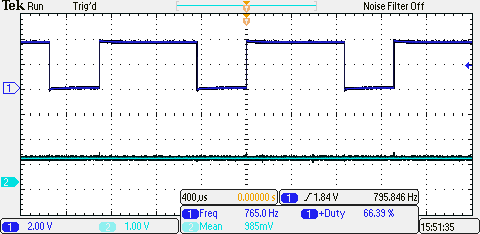
\includegraphics[width=0.475\linewidth]{../graphics/opto-low}
  }
  \subfigure[Potentiometer at \SI{5}{\kilo\ohm}]
  {
    \label{subfig:optot-high}
    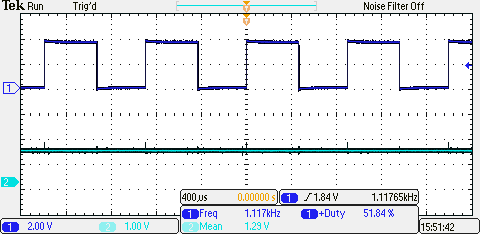
\includegraphics[width=0.475\linewidth]{../graphics/opto-high}
  }
  \caption{Timer output (top, PA1) and optocoupler voltage (bottom, PA4)}
  \label{fig:opto-traces}
\end{figure}

The values in Figs.~\ref{fig:pot-traces} and \ref{fig:opto-traces} match the output on the LCD exactly.
This is expected based on the low error from ISR overhead at this frequency range, as explained in Section~\ref{sec:test-freq}.

Using these frequencies with \eqref{eqn:555-freq} we can determine the effective value for $R_2$.
\begin{align*}
  R_2 &= {1 \over 2}\left({1.44 \over f C_1} - R_1\right) \\
  f_{low} = \SI{765}{\hertz} \implies R_2 = \SI{6.86}{\kilo\ohm} \quad 
  &\text{and} \quad f_{high} = \SI{1118}{\hertz} \implies R_2 = \SI{3.890}{\kilo\hertz}
\end{align*}
This suggests that the BJT in the 4N35 optocoupler is not in saturation when \SI{1.29}{\volt} is supplied by the microcontroller.
